\documentclass[12pt]{beamer}
\usetheme{Penn} 
\usepackage{amsmath, amssymb, amsthm, amsfonts}
\usepackage{graphicx}
\usepackage{fancyvrb}
\usepackage{verbatim}
%\usepackage{tabularx}
\usepackage{tikz}
\usepackage{animate}
\usetikzlibrary{matrix, shapes, arrows, calc, backgrounds}
\usepackage[vcentermath, enableskew]{youngtab}
\newcommand{\ZZ}{\ensuremath{\mathbb{Z}}}
\newcommand{\RR}{\ensuremath{\mathbb{R}}}
\newcommand{\PP}{\ensuremath{\mathbb{P}}}

\newcommand{\CC}{\ensuremath{\mathbb{C}}}

\newtheorem{thm}{Theorem}[section]
\newtheorem{cor}[thm]{Corollary}
\newtheorem{lem}[thm]{Lemma}
\newtheorem{prop}[thm]{Proposition}
\theoremstyle{definition}
\newtheorem{conj}[thm]{Conjecture}
\newtheorem{defn}[thm]{Definition}
\newtheorem{ex}[thm]{Example}
\newtheorem{rmk}[thm]{Remark}
\newtheorem{alg}[thm]{Algorithm}
\newtheorem{question}[thm]{Question}
\begin{document}

\author[Z. Rosen]{Zvi Rosen \\ Department of Mathematics}

\date[\today]{\today}
\title[Singular-Value Decomposition]{{\Large Diagonalization \&
 Singular-Value Decomposition}}
\institute[Dept. of Mathematics~~--~~University of Pennsylvania]{}


\frame{\titlepage}


\begin{frame}
\frametitle{Idea}
Use eigenvalues and eigenvectors to factor a matrix
into a more useful product of matrices. (Diagonalization)

Generalize this concept to non-diagonalizable matrices.
\end{frame}

\begin{frame}
\frametitle{Diagonalization}
We know how to compute eigenvalues and eigenvectors, whether
using MATLAB or by the characteristic polynomial. 

Fix a (diagonalizable) matrix $A$.
Let $D$ be a diagonal matrix whose diagonal entries are the eigenvalues 
$\lambda_1,\ldots,\lambda_n$ of $A$, and $P$ be the matrix whose columns
are the corresponding eigenvectors $x_1,\ldots,x_n$, which form a basis
of the vector space. Then:

\[ A = P D P^{-1}.\]

Why? Consider how this decomposition acts on the eigenvectors.

\end{frame}


\begin{frame}
\frametitle{Non-diagonalizable matrices}

Not every matrix is diagonalizable.

Consider the matrix
\[\begin{array}{cc}
1 & 1 \\
0 & 1 \\
\end{array}\]

This does not have a set of eigenvectors that
span the space. How can we tell?
\end{frame}


\begin{frame}
\frametitle{Application: Matrix Powers}
In many applications, we want to compute $A^M$ without
doing $M-1$ matrix multiplications. If we have a diagonalization
$A= P D P^{-1}$, then
\[ A^M = (PD P^{-1})(PD P^{-1})\cdots (PD P^{-1})\]
\[\implies A^M = P D (P^{-1}P )D (P^{-1}\cdots P) D P^{-1}) = P D^M P^{-1}.\]

Power of a diagonal matrix $D^M$ is the diagonal matrix with entries
raised to the power.
\end{frame}

\begin{frame}
\frametitle{Singular Value Decomposition}
Generalizes the notion of diagonalization for arbitrary
$m \times n$ matrices.

$A = U \Sigma V^*$ is a decomposition with $U,V$
orthogonal matrices -- corresponding to rotations --
and $\Sigma$ is a diagonal matrix ordered from largest to smallest
entries -- corresponding to stretching. The entries of $\Sigma$ are
called singular values of the matrix. They are eigenvalues of $MM*$ and
$M*M$.

\end{frame}

\begin{frame}
\frametitle{SVD: Introduction}
Strongly recommended piece on SVD: {\tt http://www.ams.org/samplings/feature-column/fcarc-svd}.

\includegraphics{svd1.gif}
\end{frame}

\begin{frame}
\frametitle{Low rank approximation}
If we throw away smaller singular values of the matrix, 
the matrix keeps doing its large-scaling operations, but instead
of shrinking some vectors, it just collapses them to zero.

\centerline{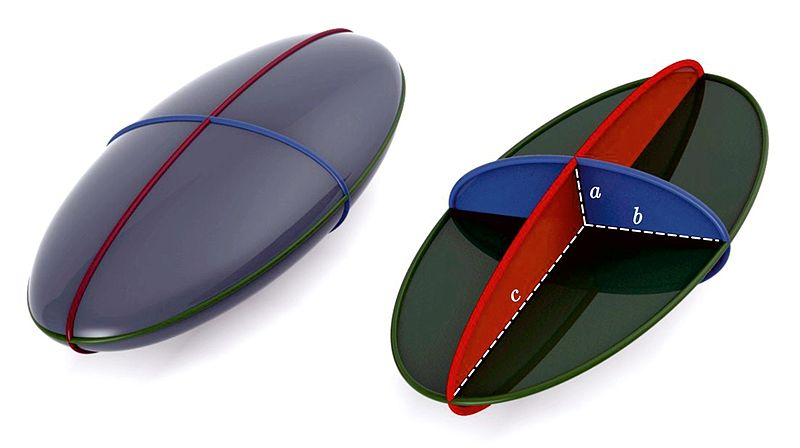
\includegraphics{ellipsoid.jpg}}

Imagine that instead of returning a vector in the larger ellipsoid at left,
it returns a vector in the oval. (Image from Wikipedia)
\end{frame}

\begin{frame}
\frametitle{Applications: Image Processing}
An image with an $m\times n$ grid of grayscale pixels can
be written as an $m \times n$ matrix with entries between
$0$ and $255$.


\end{frame}


\begin{frame}
\frametitle{Applications: Image Processing}
For instance, consider this image:

\centerline{
\includegraphics[width=.5\textwidth]{grumpy.jpg}}

This has $700 \times 700$ pixels, almost all black or white, with
some grayscale. 
\end{frame}
\end{document}
